
\section*{Problema P8.54}

\renewcommand*\thesection{8.54}
\numberwithin{equation}{section}
\numberwithin{figure}{section}

\begin{center}
    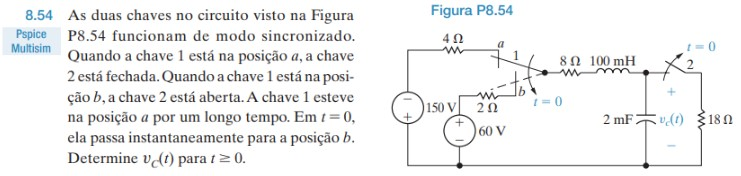
\includegraphics[scale=1.0]{P8.54.jpg}
\end{center}

O primeiro passo é identificar as condições iniciais do circuito, ou seja, as condições em $t<0$. 

\begin{figure}[hb]
    \centering
    \caption{(a) Circuito para $t<0$. (b) Circuito para $t \geq 0$.}
      \centering
      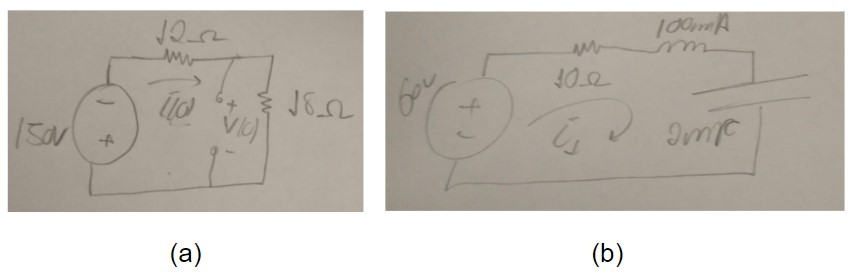
\includegraphics[scale=0.75]{P8.54-Item(a).jpg} \\
    \label{fig:8.54.1}
\end{figure}

Em $t<0$, como mostra a Figura \ref*{fig:8.54.1} (a), o circuito se reduz a um divisor de tensão resistivo. Assim, temos  

\begin{equation}\label{eq:8.54.1}
    v_C(0) = -150\frac{18}{12 + 18} = - 90 \un{V}
\end{equation}

\begin{equation}\label{eq:8.54.2}
    i_L(0) = \frac{-150}{12 + 18} = - 5 \un{A}
\end{equation}

Além disso, para identificar a condições de iniciais das derivadas de $i_L(t)$ e $v_C(t)$, usamos  

\begin{equation}\label{eq:8.54.3}
    \diff{v_C(0)}{t} = \frac{i_C(0)}{C} \logo \diff{v_C(0)}{t} = -2500 \un{V/s}
\end{equation}

\begin{equation}\label{eq:8.54.4}
    \diff{i_L(0)}{t} = \frac{v_L(0)}{L} \logo \diff{i_L(0)}{t} = \frac{0}{0.1} = 0 \un{A/s}
\end{equation}

De posse das condições inciais, aplicamos análise de malhas no circuito da Figura \ref*{fig:8.54.1} (b), obtendo

\[ -60 + Ri + L\diff{i}{t} + v_C(0) + \frac{1}{C} \int_{0}^{t}i(t) \, dt = 0 \]

Derivando com respeito a $t$,   

\[ \diff[2]{i}{t} + \frac{R}{L}\diff{i}{t} + \frac{1}{LC}i = 0 \]

A EDO acima possui equação característica dada por 

\begin{equation}\label{eq:8.54.5}
    s^2 + \frac{R}{L}s + \frac{1}{LC} = 0
\end{equation}

Substituindo com os valores do circuito da Figura \ref*{fig:8.54.1} (b),

\[ s = \frac{-(100) \pm \sqrt{(100)^2 - 4(1)(5 \cdot 10^{3})}}{2(1)} \]

\[ s = \frac{-(100) \pm j100}{2(1)} \]

\[ s_1 = -50 + j50 \un{rad/s} \quad , \quad s_2 = -50 - j50 \un{rad/s} \]

Com as duas raízes encontradas $s_1$ e $s_2$, temos que a solução geral é dada pela combinação linear

\begin{equation}\label{eq:8.54.6}
    i(t) = i_1(t) + i_2(t)
\end{equation}

Onde $i_1(t)$ e $i_2(t)$ são duas possíveis soluções para $i(t)$ dadas por  

\[ \begin{cases}
        i_1(t) = A_1e^{s_1t}  & \\
        \noalign{\vskip9pt}
        i_2(t) = A_2e^{s_2t}
    \end{cases}
\]

Diferenciando \eqref{eq:8.54.6} com respeito a $t$, temos duas equações

\[ \begin{cases}
        i(t) = A_1e^{s_1t} + A_2e^{s_2t} & \\
        \noalign{\vskip9pt}
        \diff{i(t)}{t} = A_1s_1e^{s_1t} + A_2s_2e^{s_2t}
    \end{cases}
\]

Em $t=0$, temos as condições iniciais já conhecidas em \eqref{eq:8.54.2} em \eqref{eq:8.54.4}

\[ \begin{cases}
        i(0) = A_1e^{s_10} + A_2e^{s_20} & \\
        \noalign{\vskip9pt}
        \diff{i(0)}{t} = A_1s_1e^{s_10} + A_2s_2e^{s_20}
    \end{cases}
    \logo
    \begin{cases}
        A_1 + A_2 = -5 \un{A} & \\
        \noalign{\vskip9pt}
        A_1s_1 + A_2s_2 = 0 \un{A/s}
    \end{cases}
\]

De posse dessas equações, temos o sistema linear para identificar os coeficientes $A_1$ e $A_2$

\begingroup
\renewcommand*{\arraystretch}{1.5}

\[
    \begin{bmatrix}
        1 & 1    \\
        s_1    & s_2
    \end{bmatrix}
    \begin{bmatrix}
        A_1 \\
        A_2
    \end{bmatrix}
    =
    \begin{bmatrix}
        -5 \\
        0
    \end{bmatrix} \logo
    \begin{bmatrix}
        -s_1 & -s_1    \\
        s_1    & s_2
    \end{bmatrix}
    \begin{bmatrix}
        A_1 \\
        A_2
    \end{bmatrix}
    =
    \begin{bmatrix}
        5s_1 \\
        0
    \end{bmatrix}
\]

\[
    \begin{bmatrix}
        -s_1 & -s_1    \\
        0    & s_2 - s_1
    \end{bmatrix}
    \begin{bmatrix}
        A_1 \\
        A_2
    \end{bmatrix}
    =
    \begin{bmatrix}
        5s_1 \\
        0 + 5s_1
    \end{bmatrix}
\]

\endgroup

Assim, temos  

\[ A_2 = \frac{5s_1}{s_2 - s_1} \logo  A_2 = \frac{-250 + j250}{-j100} \] 

\[ A_2 = -2.5 - j2.5 \quad , \quad A_1 = -2.5 + j2.5 \quad  \] 

Conhecidos coeficientes $A_1$ e $A_2$, bem como as raízes $s_1$ e $s_2$, temos a solução geral $v(t)$ na forma de \eqref{eq:8.54.6}

\[ i(t) = (-2.5 + j2.5)e^{(-50 + j50)t} + (-2.5 - j2.5)e^{(-50 - j50)t} \un{A} \, , \, t \geq 0  \]

Vamos remover os exponenciais complexos usando a identidade de Euler.

\[ i(t) = (-2.5 + j2.5)e^{-50t}e^{j50t} + (-2.5 - j2.5)e^{-50t}e^{-j50t} \]

\[ i(t) = (-2.5 + j2.5)e^{-50t}(\cos(50t) + j\sin(50t)) + (-2.5 - j2.5)e^{-50t}(\cos(50t) - j\sin(50t)) \]

Evidenciando o termo $e^{-50t}$ e expandindo os demais via propriedade distributiva, temos que todas 
parcelas complexas se cancelam e ficamos com

\[ \boxed{i(t) = e^{-50t}\left[-5\cos(50t) - 5\sin(50t)\right] \un{A} \, , \, t \geq 0 }  \]

Por fim, usando a relação entre corrente e tensão no capacitor de  

\[ v_C(t) = v_C(0) + \frac{1}{C} \int i(t) \, dt\]

\[ v_C(t) = -90 + \frac{1}{0.002} \int e^{-50t}\left[-5\cos(50t) - 5\sin(50t)\right] \, dt \]   

\[ v_C(t) = -90 + \frac{1}{0.002} \frac{1}{10}e^{-50t}\cos \left(50t\right) \]

\[ \boxed{v_C(t) = -90 + 50e^{-50t}\cos \left(50t\right) \un{V} \, , \, t \geq 0} \]

